% Created by tikzDevice version 0.10.1 on 2018-03-21 08:50:46
% !TEX encoding = UTF-8 Unicode
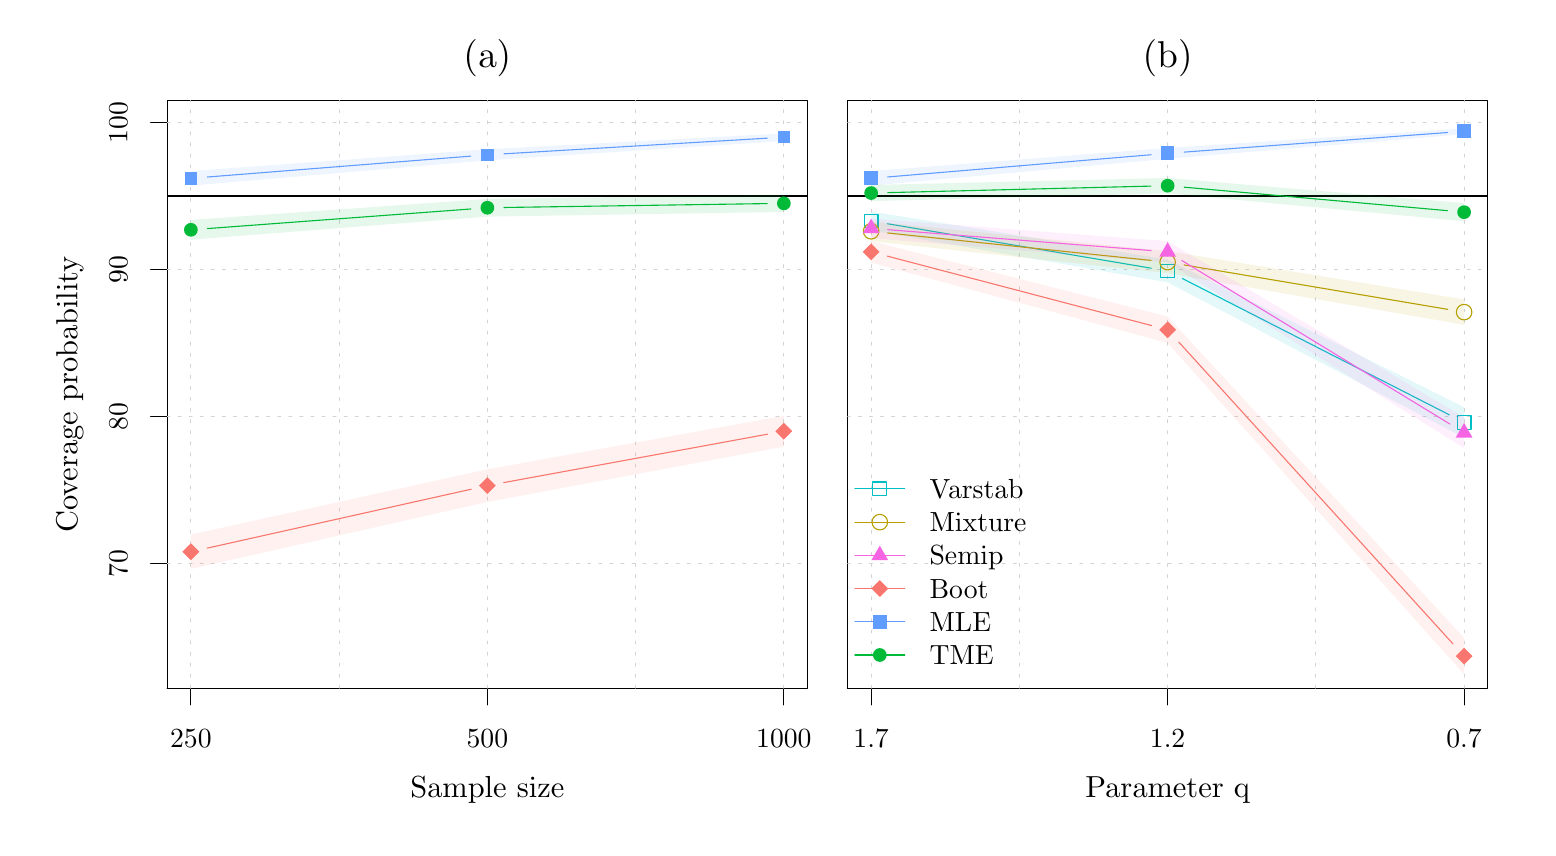
\begin{tikzpicture}[x=1pt,y=1pt]
\definecolor{fillColor}{RGB}{255,255,255}
\path[use as bounding box,fill=fillColor,fill opacity=0.00] (0,0) rectangle (542.02,289.08);
\begin{scope}
\path[clip] (  0.00,  0.00) rectangle (542.02,289.08);
\definecolor{drawColor}{RGB}{0,0,0}

\path[draw=drawColor,line width= 0.4pt,line join=round,line cap=round] ( 50.40, 95.45) -- ( 50.40,254.82);

\path[draw=drawColor,line width= 0.4pt,line join=round,line cap=round] ( 50.40, 95.45) -- ( 44.40, 95.45);

\path[draw=drawColor,line width= 0.4pt,line join=round,line cap=round] ( 50.40,148.57) -- ( 44.40,148.57);

\path[draw=drawColor,line width= 0.4pt,line join=round,line cap=round] ( 50.40,201.69) -- ( 44.40,201.69);

\path[draw=drawColor,line width= 0.4pt,line join=round,line cap=round] ( 50.40,254.82) -- ( 44.40,254.82);

\node[text=drawColor,rotate= 90.00,anchor=base,inner sep=0pt, outer sep=0pt, scale=  1.00] at ( 36.00, 95.45) {70};

\node[text=drawColor,rotate= 90.00,anchor=base,inner sep=0pt, outer sep=0pt, scale=  1.00] at ( 36.00,148.57) {80};

\node[text=drawColor,rotate= 90.00,anchor=base,inner sep=0pt, outer sep=0pt, scale=  1.00] at ( 36.00,201.69) {90};

\node[text=drawColor,rotate= 90.00,anchor=base,inner sep=0pt, outer sep=0pt, scale=  1.00] at ( 36.00,254.82) {100};

\path[draw=drawColor,line width= 0.4pt,line join=round,line cap=round] ( 50.40, 50.40) --
	(281.81, 50.40) --
	(281.81,262.68) --
	( 50.40,262.68) --
	( 50.40, 50.40);
\end{scope}
\begin{scope}
\path[clip] (  0.00,  0.00) rectangle (542.02,289.08);
\definecolor{drawColor}{RGB}{0,0,0}

\node[text=drawColor,anchor=base,inner sep=0pt, outer sep=0pt, scale=  1.10] at (166.11, 10.80) {Sample size};

\node[text=drawColor,anchor=base,inner sep=0pt, outer sep=0pt, scale=  1.35] at (166.11,274.68) {(a)};

\node[text=drawColor,rotate= 90.00,anchor=base,inner sep=0pt, outer sep=0pt, scale=  1.10] at ( 18.00,156.54) {Coverage probability};

\path[draw=drawColor,line width= 0.4pt,line join=round,line cap=round] ( 58.97, 50.40) -- (273.24, 50.40);

\path[draw=drawColor,line width= 0.4pt,line join=round,line cap=round] ( 58.97, 50.40) -- ( 58.97, 44.40);

\path[draw=drawColor,line width= 0.4pt,line join=round,line cap=round] (166.11, 50.40) -- (166.11, 44.40);

\path[draw=drawColor,line width= 0.4pt,line join=round,line cap=round] (273.24, 50.40) -- (273.24, 44.40);

\node[text=drawColor,anchor=base,inner sep=0pt, outer sep=0pt, scale=  1.00] at ( 58.97, 28.80) {250};

\node[text=drawColor,anchor=base,inner sep=0pt, outer sep=0pt, scale=  1.00] at (166.11, 28.80) {500};

\node[text=drawColor,anchor=base,inner sep=0pt, outer sep=0pt, scale=  1.00] at (273.24, 28.80) {1000};
\end{scope}
\begin{scope}
\path[clip] ( 50.40, 50.40) rectangle (281.81,262.68);
\definecolor{drawColor}{RGB}{211,211,211}

\path[draw=drawColor,line width= 0.4pt,dash pattern=on 1pt off 3pt ,line join=round,line cap=round] ( 58.97, 50.40) -- ( 58.97,262.68);

\path[draw=drawColor,line width= 0.4pt,dash pattern=on 1pt off 3pt ,line join=round,line cap=round] (112.54, 50.40) -- (112.54,262.68);

\path[draw=drawColor,line width= 0.4pt,dash pattern=on 1pt off 3pt ,line join=round,line cap=round] (166.11, 50.40) -- (166.11,262.68);

\path[draw=drawColor,line width= 0.4pt,dash pattern=on 1pt off 3pt ,line join=round,line cap=round] (219.67, 50.40) -- (219.67,262.68);

\path[draw=drawColor,line width= 0.4pt,dash pattern=on 1pt off 3pt ,line join=round,line cap=round] (273.24, 50.40) -- (273.24,262.68);

\path[draw=drawColor,line width= 0.4pt,dash pattern=on 1pt off 3pt ,line join=round,line cap=round] ( 50.40, 95.45) -- (281.81, 95.45);

\path[draw=drawColor,line width= 0.4pt,dash pattern=on 1pt off 3pt ,line join=round,line cap=round] ( 50.40,148.57) -- (281.81,148.57);

\path[draw=drawColor,line width= 0.4pt,dash pattern=on 1pt off 3pt ,line join=round,line cap=round] ( 50.40,201.69) -- (281.81,201.69);

\path[draw=drawColor,line width= 0.4pt,dash pattern=on 1pt off 3pt ,line join=round,line cap=round] ( 50.40,254.82) -- (281.81,254.82);
\definecolor{drawColor}{RGB}{0,0,0}

\path[draw=drawColor,line width= 0.4pt,line join=round,line cap=round] ( 50.40,228.26) -- (281.81,228.26);
\definecolor{drawColor}{RGB}{248,118,109}

\path[draw=drawColor,line width= 0.4pt,line join=round,line cap=round] ( 64.83,101.00) -- (160.25,122.30);

\path[draw=drawColor,line width= 0.4pt,line join=round,line cap=round] (172.01,124.69) -- (267.34,142.18);
\definecolor{fillColor}{RGB}{248,118,109}

\path[fill=fillColor] ( 55.93, 99.70) --
	( 58.97,102.74) --
	( 62.01, 99.70) --
	( 58.97, 96.66) --
	cycle;

\path[fill=fillColor] (163.07,123.60) --
	(166.11,126.64) --
	(169.14,123.60) --
	(166.11,120.57) --
	cycle;

\path[fill=fillColor] (270.20,143.26) --
	(273.24,146.30) --
	(276.28,143.26) --
	(273.24,140.22) --
	cycle;
\definecolor{fillColor}{RGB}{248,118,109}

\path[fill=fillColor,fill opacity=0.10] ( 58.97, 93.48) --
	(166.11,117.70) --
	(273.24,137.69) --
	(273.24,148.83) --
	(166.11,129.50) --
	( 58.97,105.92) --
	cycle;
\definecolor{drawColor}{RGB}{97,156,255}

\path[draw=drawColor,line width= 0.4pt,line join=round,line cap=round] ( 64.95,235.11) -- (160.13,242.66);

\path[draw=drawColor,line width= 0.4pt,line join=round,line cap=round] (172.10,243.49) -- (267.25,249.15);
\definecolor{fillColor}{RGB}{97,156,255}

\path[fill=fillColor] ( 56.72,232.38) --
	( 61.22,232.38) --
	( 61.22,236.88) --
	( 56.72,236.88) --
	cycle;

\path[fill=fillColor] (163.86,240.88) --
	(168.36,240.88) --
	(168.36,245.38) --
	(163.86,245.38) --
	cycle;

\path[fill=fillColor] (270.99,247.26) --
	(275.49,247.26) --
	(275.49,251.76) --
	(270.99,251.76) --
	cycle;
\definecolor{fillColor}{RGB}{97,156,255}

\path[fill=fillColor,fill opacity=0.10] ( 58.97,232.01) --
	(166.11,241.12) --
	(273.24,248.14) --
	(273.24,250.87) --
	(166.11,245.14) --
	( 58.97,237.25) --
	cycle;
\definecolor{drawColor}{RGB}{0,186,56}

\path[draw=drawColor,line width= 0.4pt,line join=round,line cap=round] ( 64.95,216.48) -- (160.12,223.56);

\path[draw=drawColor,line width= 0.4pt,line join=round,line cap=round] (172.11,224.10) -- (267.24,225.51);
\definecolor{fillColor}{RGB}{0,186,56}

\path[fill=fillColor] ( 58.97,216.04) circle (  2.48);

\path[fill=fillColor] (166.11,224.01) circle (  2.48);

\path[fill=fillColor] (273.24,225.60) circle (  2.48);
\definecolor{fillColor}{RGB}{0,186,56}

\path[fill=fillColor,fill opacity=0.10] ( 58.97,212.48) --
	(166.11,220.81) --
	(273.24,222.48) --
	(273.24,228.72) --
	(166.11,227.20) --
	( 58.97,219.60) --
	cycle;
\end{scope}
\begin{scope}
\path[clip] (  0.00,  0.00) rectangle (542.02,289.08);
\definecolor{drawColor}{RGB}{0,0,0}

\path[draw=drawColor,line width= 0.4pt,line join=round,line cap=round] (296.21, 50.40) --
	(527.62, 50.40) --
	(527.62,262.68) --
	(296.21,262.68) --
	(296.21, 50.40);
\end{scope}
\begin{scope}
\path[clip] (295.01, 49.20) rectangle (540.83,275.88);
\definecolor{drawColor}{RGB}{0,0,0}

\node[text=drawColor,rotate= 90.00,anchor=base,inner sep=0pt, outer sep=0pt, scale=  1.00] at (257.81,156.54) { };
\end{scope}
\begin{scope}
\path[clip] (  0.00,  0.00) rectangle (542.02,289.08);
\definecolor{drawColor}{RGB}{0,0,0}

\path[draw=drawColor,line width= 0.4pt,line join=round,line cap=round] (304.78, 50.40) -- (519.05, 50.40);

\path[draw=drawColor,line width= 0.4pt,line join=round,line cap=round] (304.78, 50.40) -- (304.78, 44.40);

\path[draw=drawColor,line width= 0.4pt,line join=round,line cap=round] (411.92, 50.40) -- (411.92, 44.40);

\path[draw=drawColor,line width= 0.4pt,line join=round,line cap=round] (519.05, 50.40) -- (519.05, 44.40);

\node[text=drawColor,anchor=base,inner sep=0pt, outer sep=0pt, scale=  1.00] at (304.78, 28.80) {1.7};

\node[text=drawColor,anchor=base,inner sep=0pt, outer sep=0pt, scale=  1.00] at (411.92, 28.80) {1.2};

\node[text=drawColor,anchor=base,inner sep=0pt, outer sep=0pt, scale=  1.00] at (519.05, 28.80) {0.7};

\node[text=drawColor,anchor=base,inner sep=0pt, outer sep=0pt, scale=  1.10] at (411.92, 10.80) {Parameter q};

\node[text=drawColor,anchor=base,inner sep=0pt, outer sep=0pt, scale=  1.35] at (411.92,274.68) {(b)};
\end{scope}
\begin{scope}
\path[clip] (296.21, 50.40) rectangle (527.62,262.68);
\definecolor{drawColor}{RGB}{211,211,211}

\path[draw=drawColor,line width= 0.4pt,dash pattern=on 1pt off 3pt ,line join=round,line cap=round] (304.78, 50.40) -- (304.78,262.68);

\path[draw=drawColor,line width= 0.4pt,dash pattern=on 1pt off 3pt ,line join=round,line cap=round] (358.35, 50.40) -- (358.35,262.68);

\path[draw=drawColor,line width= 0.4pt,dash pattern=on 1pt off 3pt ,line join=round,line cap=round] (411.92, 50.40) -- (411.92,262.68);

\path[draw=drawColor,line width= 0.4pt,dash pattern=on 1pt off 3pt ,line join=round,line cap=round] (465.49, 50.40) -- (465.49,262.68);

\path[draw=drawColor,line width= 0.4pt,dash pattern=on 1pt off 3pt ,line join=round,line cap=round] (519.05, 50.40) -- (519.05,262.68);

\path[draw=drawColor,line width= 0.4pt,dash pattern=on 1pt off 3pt ,line join=round,line cap=round] (296.21, 95.45) -- (527.62, 95.45);

\path[draw=drawColor,line width= 0.4pt,dash pattern=on 1pt off 3pt ,line join=round,line cap=round] (296.21,148.57) -- (527.62,148.57);

\path[draw=drawColor,line width= 0.4pt,dash pattern=on 1pt off 3pt ,line join=round,line cap=round] (296.21,201.69) -- (527.62,201.69);

\path[draw=drawColor,line width= 0.4pt,dash pattern=on 1pt off 3pt ,line join=round,line cap=round] (296.21,254.82) -- (527.62,254.82);
\definecolor{drawColor}{RGB}{0,0,0}

\path[draw=drawColor,line width= 0.4pt,line join=round,line cap=round] (296.21,228.26) -- (527.62,228.26);
\definecolor{drawColor}{RGB}{0,191,196}

\path[draw=drawColor,line width= 0.4pt,line join=round,line cap=round] (310.70,218.23) -- (406.00,202.16);

\path[draw=drawColor,line width= 0.4pt,line join=round,line cap=round] (417.26,198.43) -- (513.71,149.18);

\path[draw=drawColor,line width= 0.4pt,line join=round,line cap=round] (302.29,216.73) rectangle (307.28,221.72);

\path[draw=drawColor,line width= 0.4pt,line join=round,line cap=round] (409.43,198.67) rectangle (414.41,203.66);

\path[draw=drawColor,line width= 0.4pt,line join=round,line cap=round] (516.56,143.95) rectangle (521.55,148.94);
\definecolor{fillColor}{RGB}{0,191,196}

\path[fill=fillColor,fill opacity=0.10] (304.78,215.80) --
	(411.92,197.04) --
	(519.05,140.93) --
	(519.05,151.96) --
	(411.92,205.29) --
	(304.78,222.65) --
	cycle;
\definecolor{drawColor}{RGB}{183,159,0}

\path[draw=drawColor,line width= 0.4pt,line join=round,line cap=round] (310.75,214.89) -- (405.95,204.97);

\path[draw=drawColor,line width= 0.4pt,line join=round,line cap=round] (417.84,203.35) -- (513.14,187.29);

\path[draw=drawColor,line width= 0.4pt,line join=round,line cap=round] (304.78,215.51) circle (  2.81);

\path[draw=drawColor,line width= 0.4pt,line join=round,line cap=round] (411.92,204.35) circle (  2.81);

\path[draw=drawColor,line width= 0.4pt,line join=round,line cap=round] (519.05,186.29) circle (  2.81);
\definecolor{fillColor}{RGB}{183,159,0}

\path[fill=fillColor,fill opacity=0.10] (304.78,211.92) --
	(411.92,200.34) --
	(519.05,181.70) --
	(519.05,190.88) --
	(411.92,208.36) --
	(304.78,219.09) --
	cycle;
\definecolor{drawColor}{RGB}{245,100,227}

\path[draw=drawColor,line width= 0.4pt,line join=round,line cap=round] (310.76,216.09) -- (405.94,208.54);

\path[draw=drawColor,line width= 0.4pt,line join=round,line cap=round] (417.04,204.95) -- (513.93,145.85);
\definecolor{fillColor}{RGB}{245,100,227}

\path[fill=fillColor] (304.78,220.07) --
	(307.81,214.82) --
	(301.75,214.82) --
	cycle;

\path[fill=fillColor] (411.92,211.57) --
	(414.95,206.32) --
	(408.89,206.32) --
	cycle;

\path[fill=fillColor] (519.05,146.23) --
	(522.08,140.98) --
	(516.02,140.98) --
	cycle;
\definecolor{fillColor}{RGB}{245,100,227}

\path[fill=fillColor,fill opacity=0.10] (304.78,213.03) --
	(411.92,204.19) --
	(519.05,137.14) --
	(519.05,148.31) --
	(411.92,211.95) --
	(304.78,220.11) --
	cycle;
\definecolor{drawColor}{RGB}{248,118,109}

\path[draw=drawColor,line width= 0.4pt,line join=round,line cap=round] (310.59,206.54) -- (406.12,181.44);

\path[draw=drawColor,line width= 0.4pt,line join=round,line cap=round] (415.95,175.47) -- (515.02, 66.42);
\definecolor{fillColor}{RGB}{248,118,109}

\path[fill=fillColor] (301.75,208.07) --
	(304.78,211.11) --
	(307.82,208.07) --
	(304.78,205.03) --
	cycle;

\path[fill=fillColor] (408.88,179.91) --
	(411.92,182.95) --
	(414.96,179.91) --
	(411.92,176.88) --
	cycle;

\path[fill=fillColor] (516.02, 61.98) --
	(519.05, 65.02) --
	(522.09, 61.98) --
	(519.05, 58.94) --
	cycle;
\definecolor{fillColor}{RGB}{248,118,109}

\path[fill=fillColor,fill opacity=0.10] (304.78,204.19) --
	(411.92,175.15) --
	(519.05, 55.40) --
	(519.05, 68.56) --
	(411.92,184.68) --
	(304.78,211.95) --
	cycle;
\definecolor{drawColor}{RGB}{97,156,255}

\path[draw=drawColor,line width= 0.4pt,line join=round,line cap=round] (310.76,235.13) -- (405.94,243.16);

\path[draw=drawColor,line width= 0.4pt,line join=round,line cap=round] (417.90,244.11) -- (513.07,251.19);
\definecolor{fillColor}{RGB}{97,156,255}

\path[fill=fillColor] (302.31,232.16) --
	(307.26,232.16) --
	(307.26,237.11) --
	(302.31,237.11) --
	cycle;

\path[fill=fillColor] (409.44,241.19) --
	(414.39,241.19) --
	(414.39,246.14) --
	(409.44,246.14) --
	cycle;

\path[fill=fillColor] (516.58,249.16) --
	(521.53,249.16) --
	(521.53,254.11) --
	(516.58,254.11) --
	cycle;
\definecolor{fillColor}{RGB}{97,156,255}

\path[fill=fillColor,fill opacity=0.10] (304.78,232.01) --
	(411.92,241.70) --
	(519.05,250.57) --
	(519.05,252.69) --
	(411.92,245.62) --
	(304.78,237.25) --
	cycle;
\definecolor{drawColor}{RGB}{0,186,56}

\path[draw=drawColor,line width= 0.4pt,line join=round,line cap=round] (310.78,229.47) -- (405.92,231.83);

\path[draw=drawColor,line width= 0.4pt,line join=round,line cap=round] (417.89,231.44) -- (513.08,222.95);
\definecolor{fillColor}{RGB}{0,186,56}

\path[fill=fillColor] (304.78,229.32) circle (  2.48);

\path[fill=fillColor] (411.92,231.97) circle (  2.48);

\path[fill=fillColor] (519.05,222.41) circle (  2.48);
\definecolor{fillColor}{RGB}{0,186,56}

\path[fill=fillColor,fill opacity=0.10] (304.78,226.39) --
	(411.92,229.20) --
	(519.05,219.14) --
	(519.05,225.69) --
	(411.92,234.75) --
	(304.78,232.24) --
	cycle;
\definecolor{drawColor}{RGB}{0,191,196}

\path[draw=drawColor,line width= 0.4pt,line join=round,line cap=round] (298.91,122.40) -- (316.91,122.40);
\definecolor{drawColor}{RGB}{183,159,0}

\path[draw=drawColor,line width= 0.4pt,line join=round,line cap=round] (298.91,110.40) -- (316.91,110.40);
\definecolor{drawColor}{RGB}{245,100,227}

\path[draw=drawColor,line width= 0.4pt,line join=round,line cap=round] (298.91, 98.40) -- (316.91, 98.40);
\definecolor{drawColor}{RGB}{248,118,109}

\path[draw=drawColor,line width= 0.4pt,line join=round,line cap=round] (298.91, 86.40) -- (316.91, 86.40);
\definecolor{drawColor}{RGB}{97,156,255}

\path[draw=drawColor,line width= 0.4pt,line join=round,line cap=round] (298.91, 74.40) -- (316.91, 74.40);
\definecolor{drawColor}{RGB}{0,186,56}

\path[draw=drawColor,line width= 0.4pt,line join=round,line cap=round] (298.91, 62.40) -- (316.91, 62.40);
\definecolor{drawColor}{RGB}{0,191,196}

\path[draw=drawColor,line width= 0.4pt,line join=round,line cap=round] (305.42,119.91) rectangle (310.41,124.89);
\definecolor{drawColor}{RGB}{183,159,0}

\path[draw=drawColor,line width= 0.4pt,line join=round,line cap=round] (307.91,110.40) circle (  2.81);
\definecolor{fillColor}{RGB}{245,100,227}

\path[fill=fillColor] (307.91,101.90) --
	(310.94, 96.65) --
	(304.88, 96.65) --
	cycle;
\definecolor{fillColor}{RGB}{248,118,109}

\path[fill=fillColor] (304.88, 86.40) --
	(307.91, 89.44) --
	(310.95, 86.40) --
	(307.91, 83.36) --
	cycle;
\definecolor{fillColor}{RGB}{97,156,255}

\path[fill=fillColor] (305.44, 71.93) --
	(310.39, 71.93) --
	(310.39, 76.88) --
	(305.44, 76.88) --
	cycle;
\definecolor{fillColor}{RGB}{0,186,56}

\path[fill=fillColor] (307.91, 62.40) circle (  2.48);
\definecolor{drawColor}{RGB}{0,0,0}

\node[text=drawColor,anchor=base west,inner sep=0pt, outer sep=0pt, scale=  1.00] at (325.91,118.96) {Varstab};

\node[text=drawColor,anchor=base west,inner sep=0pt, outer sep=0pt, scale=  1.00] at (325.91,106.96) {Mixture};

\node[text=drawColor,anchor=base west,inner sep=0pt, outer sep=0pt, scale=  1.00] at (325.91, 94.96) {Semip};

\node[text=drawColor,anchor=base west,inner sep=0pt, outer sep=0pt, scale=  1.00] at (325.91, 82.96) {Boot};

\node[text=drawColor,anchor=base west,inner sep=0pt, outer sep=0pt, scale=  1.00] at (325.91, 70.96) {MLE};

\node[text=drawColor,anchor=base west,inner sep=0pt, outer sep=0pt, scale=  1.00] at (325.91, 58.96) {TME};
\end{scope}
\end{tikzpicture}
